%%
%% This is file `sample-sigplan.tex',
%% generated with the docstrip utility.
%%
%% The original source files were:
%%
%% samples.dtx  (with options: `all,proceedings,bibtex,sigplan')
%% 
%% IMPORTANT NOTICE:
%% 
%% For the copyright see the source file.
%% 
%% Any modified versions of this file must be renamed
%% with new filenames distinct from sample-sigplan.tex.
%% 
%% For distribution of the original source see the terms
%% for copying and modification in the file samples.dtx.
%% 
%% This generated file may be distributed as long as the
%% original source files, as listed above, are part of the
%% same distribution. (The sources need not necessarily be
%% in the same archive or directory.)
%%
%%
%% Commands for TeXCount
%TC:macro \cite [option:text,text]
%TC:macro \citep [option:text,text]
%TC:macro \citet [option:text,text]
%TC:envir table 0 1
%TC:envir table* 0 1
%TC:envir tabular [ignore] word
%TC:envir displaymath 0 word
%TC:envir math 0 word
%TC:envir comment 0 0
%%
%%
%% The first command in your LaTeX source must be the \documentclass
%% command.
%%
%% For submission and review of your manuscript please change the
%% command to \documentclass[manuscript, screen, review]{acmart}.
%%
%% When submitting camera ready or to TAPS, please change the command
%% to \documentclass[sigconf]{acmart} or whichever template is required
%% for your publication.
%%
%%
\documentclass[sigplan,screen]{acmart}

%%
%% \BibTeX command to typeset BibTeX logo in the docs
\AtBeginDocument{%
  \providecommand\BibTeX{{%
    Bib\TeX}}}

%% Rights management information.  This information is sent to you
%% when you complete the rights form.  These commands have SAMPLE
%% values in them; it is your responsibility as an author to replace
%% the commands and values with those provided to you when you
%% complete the rights form.
\setcopyright{acmlicensed}
\copyrightyear{2025}
\acmYear{2025}
\acmDOI{XXXXXXX.XXXXXXX}

%% These commands are for a PROCEEDINGS abstract or paper.
\acmConference[MLOPs y Puesta en Producción]{Make sure to enter the correct
  conference title from your rights confirmation emai}{Agosto 31-08,
  2025}{Santa Cruz, Bolivia}
%%
%%  Uncomment \acmBooktitle if the title of the proceedings is different
%%  from ``Proceedings of ...''!
%%
%%\acmBooktitle{Woodstock '18: ACM Symposium on Neural Gaze Detection,
%%  June 03--05, 2018, Woodstock, NY}
\acmISBN{978-1-4503-XXXX-X/18/06}


%%
%% Submission ID.
%% Use this when submitting an article to a sponsored event. You'll
%% receive a unique submission ID from the organizers
%% of the event, and this ID should be used as the parameter to this command.
%%\acmSubmissionID{123-A56-BU3}

%%
%% For managing citations, it is recommended to use bibliography
%% files in BibTeX format.
%%
%% You can then either use BibTeX with the ACM-Reference-Format style,
%% or BibLaTeX with the acmnumeric or acmauthoryear sytles, that include
%% support for advanced citation of software artefact from the
%% biblatex-software package, also separately available on CTAN.
%%
%% Look at the sample-*-biblatex.tex files for templates showcasing
%% the biblatex styles.
%%

%%
%% The majority of ACM publications use numbered citations and
%% references.  The command \citestyle{authoryear} switches to the
%% "author year" style.
%%
%% If you are preparing content for an event
%% sponsored by ACM SIGGRAPH, you must use the "author year" style of
%% citations and references.
%% Uncommenting
%% the next command will enable that style.
%%\citestyle{acmauthoryear}
\usepackage{tabularx}
\usepackage{graphicx}
\usepackage[spanish]{babel}

\newcommand{\staricon}[1]{
    \begin{tikzpicture}[scale=#1]
        \filldraw[fill=yellow, draw=black] 
        (0,0) -- (0.2,0.6) -- (0.6,0.6) -- (0.3,0.9) -- (0.4,1.4) -- (0,1.1) -- (-0.4,1.4) -- (-0.3,0.9) -- (-0.6,0.6) -- (-0.2,0.6) -- cycle;
    \end{tikzpicture}
}

%%
%% end of the preamble, start of the body of the document source.
\begin{document}

%%
%% The "title" command has an optional parameter,
%% allowing the author to define a "short title" to be used in page headers.
\title{PROYECTO FINAL: MLOPs y Puesta en Producción}

%%
%% The "author" command and its associated commands are used to define
%% the authors and their affiliations.
%% Of note is the shared affiliation of the first two authors, and the
%% "authornote" and "authornotemark" commands
%% used to denote shared contribution to the research.
% \author{Bravo Peña}
% \author{Darlyn}
% \affiliation{
%   \institution{UAGRM}
%   \city{Santa Cruz}
%   \country{Bolivia}
% }
% \email{contact@bpdarlyn.com}

% \author{Torrejón Mendez}
% \author{Joel Gabriel}
% \affiliation{
%   \institution{UAGRM}
%   \city{Santa Cruz}
%   \country{Bolivia}
% }
% \email{joel.torrejon.mendez@gmail.com}

% \author{Valle Tamayo}
% \author{Brandon Jason}
% \affiliation{
%   \institution{UAGRM}
%   \city{Santa Cruz}
%   \country{Bolivia}}
% \email{bjvtamayo78@gmail.com}

% \author{Vega Guerra}
% \author{Giovanni Heriberto}
% \affiliation{
%   \institution{UAGRM}
%   \city{Santa Cruz}
%   \country{Bolivia}}
% \email{zxvega@gmail.com}

\author{Bravo Peña Darlyn \and Torrejón Mendez Joel Gabriel \and Valle Tamayo Brandon Jason \and Vega Guerra Giovanni Heriberto}
\affiliation{
  \institution{UAGRM}
  \city{Santa Cruz}
  \country{Bolivia}
}
\email{contact@bpdarlyn.com, joel.torrejon.mendez@gmail.com, bjvtamayo78@gmail.com, zxvega@gmail.com}

%%
%% By default, the full list of authors will be used in the page
%% headers. Often, this list is too long, and will overlap
%% other information printed in the page headers. This command allows
%% the author to define a more concise list
%% of authors' names for this purpose.
\renewcommand{\shortauthors}{Bravo - Torrejón - Valle - Vega}

%%
%% The code below is generated by the tool at http://dl.acm.org/ccs.cfm.
%% Please copy and paste the code instead of the example below.
%%
% \begin{CCSXML}
% <ccs2012>
%  <concept>
%   <concept_id>00000000.0000000.0000000</concept_id>
%   <concept_desc>Do Not Use This Code, Generate the Correct Terms for Your Paper</concept_desc>
%   <concept_significance>500</concept_significance>
%  </concept>
%  <concept>
%   <concept_id>00000000.00000000.00000000</concept_id>
%   <concept_desc>Do Not Use This Code, Generate the Correct Terms for Your Paper</concept_desc>
%   <concept_significance>300</concept_significance>
%  </concept>
%  <concept>
%   <concept_id>00000000.00000000.00000000</concept_id>
%   <concept_desc>Do Not Use This Code, Generate the Correct Terms for Your Paper</concept_desc>
%   <concept_significance>100</concept_significance>
%  </concept>
%  <concept>
%   <concept_id>00000000.00000000.00000000</concept_id>
%   <concept_desc>Do Not Use This Code, Generate the Correct Terms for Your Paper</concept_desc>
%   <concept_significance>100</concept_significance>
%  </concept>
% </ccs2012>
% \end{CCSXML}

% \ccsdesc[500]{Do Not Use This Code~Generate the Correct Terms for Your Paper}
% \ccsdesc[300]{Do Not Use This Code~Generate the Correct Terms for Your Paper}
% \ccsdesc{Do Not Use This Code~Generate the Correct Terms for Your Paper}
% \ccsdesc[100]{Do Not Use This Code~Generate the Correct Terms for Your Paper}

%%
%% Keywords. The author(s) should pick words that accurately describe
%% the work being presented. Separate the keywords with commas.
% \keywords{Do, Not, Us, This, Code, Put, the, Correct, Terms, for,
%   Your, Paper}
%% A "teaser" image appears between the author and affiliation
%% information and the body of the document, and typically spans the
%% page.
\begin{teaserfigure}
  
\includegraphics[width=\textwidth]{images/logo_soe.png}
  \Description{UAGRM SOE LOGO}
  \label{fig:teaser}
\end{teaserfigure}

\received{30 August 2025}
\received[revised]{30 August 2025}
\received[accepted]{5 June 2009}

%%
%% This command processes the author and affiliation and title
%% information and builds the first part of the formatted document.
\maketitle

% Document content
\section{Introducción}
El propósito de este artículo es de hacer una investigación sobre las
opciones de software Api Gateway, a efectos de este artículo elegimos
dos opciones: Kong y AWS, para determinar cuál es
la mejor opción para un proyecto de desarrollo de software. Se hará un
análisis comparativo de las características de ambos productos, sus pros
y contras, y se determinará cuál es la mejor opción para un proyecto de
desarrollo de software. Se espera que este artículo sea útil para
desarrolladores de software que estén considerando utilizar un Api Gateway.

\section{Datos}

El proyecto utiliza como fuente principal el conjunto de datos \textbf{UTKFace},
reconocido en la literatura por su aplicación en tareas de clasificación de género y 
estimación de edad. Este dataset contiene aproximadamente 20.000 imágenes faciales en formato RGB con 
dimensiones cercanas a 200×200 píxeles. 
Cada archivo está anotado siguiendo el patrón \textit{edad\_género\_raza\_timestamp.jpg}, 
lo que permite extraer de manera automática las etiquetas de edad (en años) y género (0 = femenino, 1 = masculino).

\subsection{Fuente y Organización}
La descarga y organización inicial del dataset se realizó con un script automatizado (\texttt{download\_utkface.py}), 
que obtiene los archivos desde Kaggle y, en caso de fallo, genera un subconjunto sintético para pruebas rápidas. 
Posteriormente, el script \texttt{prepare\_utkface.py} extrae las anotaciones y genera un archivo \texttt{labels.csv}, 
que contiene de forma tabular las columnas \textit{filename}, \textit{age} y \textit{gender}.

\subsection{Procesamiento y Transformaciones}
Durante el proceso de preparación se aplicaron varias transformaciones para garantizar la calidad de los datos:

\begin{itemize}
  \item \textbf{Limpieza y filtrado}: se descartaron archivos que no cumplían con el patrón de nomenclatura o presentaban errores de lectura.
  \item \textbf{Redimensionamiento}: las imágenes fueron escaladas a 160×160 píxeles, en concordancia con la entrada requerida por el modelo.
  \item \textbf{Normalización}: los valores de píxeles fueron ajustados al rango [0,1] para estabilizar el entrenamiento.
  \item \textbf{Data augmentation}: se aplicó un pipeline de aumentos ligeros mediante rotaciones, volteos, zoom, traslaciones, ajustes de contraste y correcciones aleatorias de gamma. Este esquema se implementó como una capa inicial dentro del modelo en Keras, garantizando variaciones adicionales de los datos en cada época de entrenamiento.
\end{itemize}

\subsection{Limitaciones}
A pesar de su utilidad, el dataset presenta algunas limitaciones relevantes:

\begin{itemize}
  \item \textbf{Desbalance etario}: predominan ejemplos de edades jóvenes y adultas, mientras que los grupos etarios extremos están poco representados.
  \item \textbf{Diversidad poblacional limitada}: UTKFace no refleja la composición étnica de la población boliviana, lo cual puede afectar la generalización del modelo.
  \item \textbf{Posible ruido en las etiquetas}: la edad se infiere del nombre del archivo y no siempre corresponde a un dato verificado.
\end{itemize}

\subsection{Perspectiva Futura}
Si bien UTKFace constituye la base de esta primera iteración, 
se contempla la incorporación del dataset \textbf{QMUL-SurvFace} en futuros trabajos. 
Dicho conjunto incluye imágenes en escenarios de vigilancia no controlada, lo que permitiría enriquecer 
la robustez del sistema y acercar el modelo a contextos reales de aplicación.

\section{Métodos}

El enfoque propuesto se basa en un modelo de \textbf{aprendizaje profundo multitarea}, diseñado para resolver simultáneamente la estimación de edad (regresión) y la clasificación de género (clasificación binaria). La arquitectura aprovecha el paradigma de \textit{transfer learning}, utilizando como base una red preentrenada en ImageNet y añadiendo cabezales especializados para cada tarea.

\subsection{Arquitectura del modelo}
La red está compuesta por tres bloques principales:
\begin{itemize}
  \item \textbf{Bloque de aumento de datos}: implementado como una capa secuencial en Keras que aplica transformaciones ligeras (volteos horizontales, rotaciones, zoom, traslaciones, ajustes de contraste y variaciones aleatorias de gamma). Este componente mejora la capacidad de generalización del modelo frente a condiciones no controladas de captura de imágenes.
  \item \textbf{Bloque de extracción de características}: se emplea \textbf{MobileNetV2} como \textit{backbone}, con pesos iniciales de ImageNet. Esta arquitectura fue seleccionada por su eficiencia computacional y bajo número de parámetros, lo que la hace adecuada para despliegue en entornos con recursos limitados.
  \item \textbf{Bloque de predicción multitarea}: tras una capa de \textit{Global Average Pooling} y \textit{Dropout}, se añaden dos salidas: una capa densa lineal para la predicción de edad (pérdida: \texttt{MAE}), y una capa densa sigmoide para la clasificación de género (pérdida: \texttt{binary\_crossentropy}).
\end{itemize}

\subsection{Entrenamiento y optimización}
El proceso de entrenamiento se realizó en dos fases:
\begin{enumerate}
  \item \textbf{Fase de extracción de características}: el backbone MobileNetV2 permaneció congelado, entrenando únicamente las capas superiores añadidas. Se utilizó el optimizador Adam con tasa de aprendizaje $1\mathrm{e}{-3}$, aplicando \textit{early stopping} para prevenir sobreajuste.
  \item \textbf{Fase de ajuste fino (fine-tuning)}: se descongelaron las últimas 20 capas del backbone, reduciendo la tasa de aprendizaje a $1\mathrm{e}{-4}$ para permitir una adaptación gradual de los pesos preentrenados al dominio de rostros.
\end{enumerate}

Las métricas principales utilizadas fueron \textbf{accuracy} para la tarea de género y \textbf{MAE} (Mean Absolute Error) para la predicción de edad. El entrenamiento se realizó en lotes de tamaño 32 durante un máximo de 16 épocas, con división de validación del 10\% sobre el dataset.

\subsection{Gestión de experimentos}
Para el seguimiento de experimentos y control de versiones de modelos se empleó \textbf{MLflow}. En cada ejecución se registraron parámetros de entrenamiento, métricas de desempeño y artefactos asociados (curvas de aprendizaje, matriz de confusión y exportación del modelo en formato ONNX). Este enfoque permitió comparar la fase inicial de entrenamiento con la etapa de fine-tuning, así como almacenar los resultados de forma reproducible.

\subsection{Alternativas consideradas}
Si bien MobileNetV2 fue seleccionado por su balance entre precisión y eficiencia, se consideran varias alternativas para futuras iteraciones:
\begin{itemize}
  \item \textbf{EfficientNet}: por su capacidad de escalar en profundidad y resolución con menor costo computacional.
  \item \textbf{ResNet-50}: ampliamente utilizada en reconocimiento facial, aunque con mayor carga de parámetros.
  \item \textbf{Modelos específicos para estimación de edad}: arquitecturas diseñadas para tareas demográficas que podrían mejorar el desempeño en la predicción de edades extremas.
\end{itemize}

Este planteamiento metodológico asegura una base sólida para abordar el problema de clasificación de género y estimación de edad, al tiempo que sienta las bases para futuras mejoras y experimentación en escenarios más desafiantes.

\section{Despliegue}

Para llevar el modelo a producción, se diseñó una arquitectura distribuida basada en contenedores Docker y buenas prácticas de MLOps. A continuación se detalla su estructura:

\subsection{Arquitectura del sistema}
El sistema está organizado en cuatro servicios principales, cada uno desplegado en un contenedor Docker coordinado mediante \texttt{docker-compose}:

\begin{itemize}
  \item \textbf{db}: base de datos MySQL que almacena los experimentos, los metadatos de entrenamiento y los embeddings faciales.
  \item \textbf{mlflow}: servidor de seguimiento MLflow para registrar ejecuciones, métricas, artefactos y modelos entrenados.
  \item \textbf{trainer}: entorno para entrenamiento y pruebas del modelo, incluyendo scripts para generación de experimentos y guardado de modelos.
  \item \textbf{face-api}: API REST basada en \texttt{FastAPI} para ofrecer el servicio de predicción (edad y género) en tiempo real.
\end{itemize}

\subsection{Seguimiento de experimentos y registro de modelos}
Durante la fase de entrenamiento se integró \textbf{MLflow} como plataforma central de seguimiento. Cada ejecución (\textit{run}) dentro del experimento \texttt{AgeGender-UTKFace} registró:

\begin{itemize}
  \item \textbf{Parámetros}: configuración de entrenamiento (número de épocas, tamaño de lote, tasa de aprendizaje).
  \item \textbf{Métricas}: error absoluto medio (MAE) para la predicción de edad y precisión (accuracy) para la clasificación de género, en dos fases distintas (entrenamiento inicial y fine-tuning).
  \item \textbf{Artefactos}: curvas de entrenamiento, matriz de confusión, el modelo exportado en formato TensorFlow y su conversión a ONNX.
\end{itemize}

\begin{figure}[h]
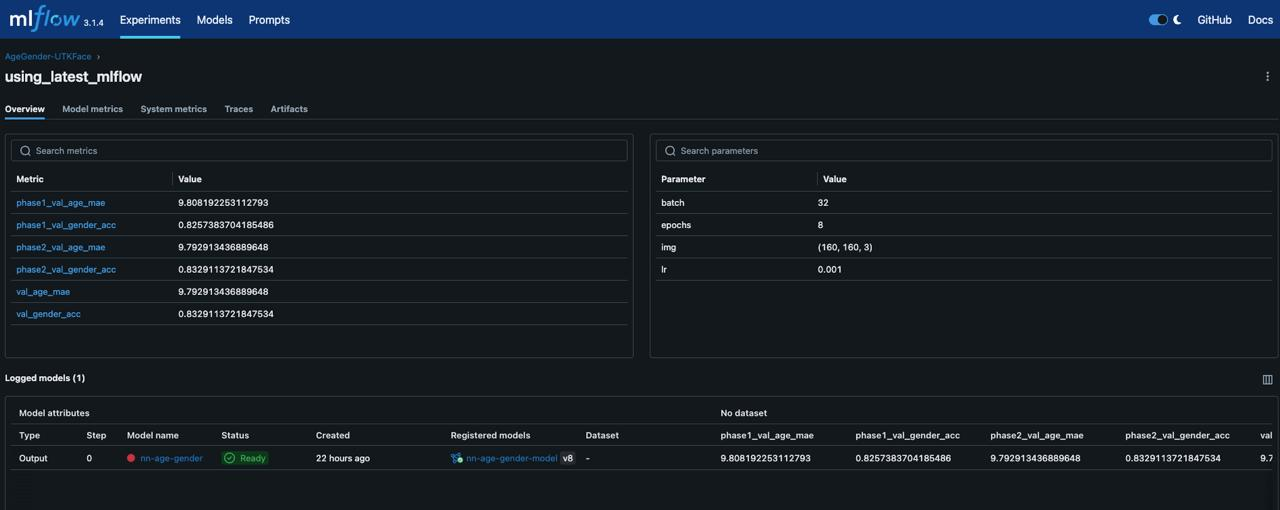
\includegraphics[width=0.5\textwidth]{images/mlflow_metrics.jpeg}
\centering
\caption{Registro de métricas de entrenamiento en MLflow.}
\label{fig:mlflow-metrics}
\end{figure}

\begin{figure}[h]
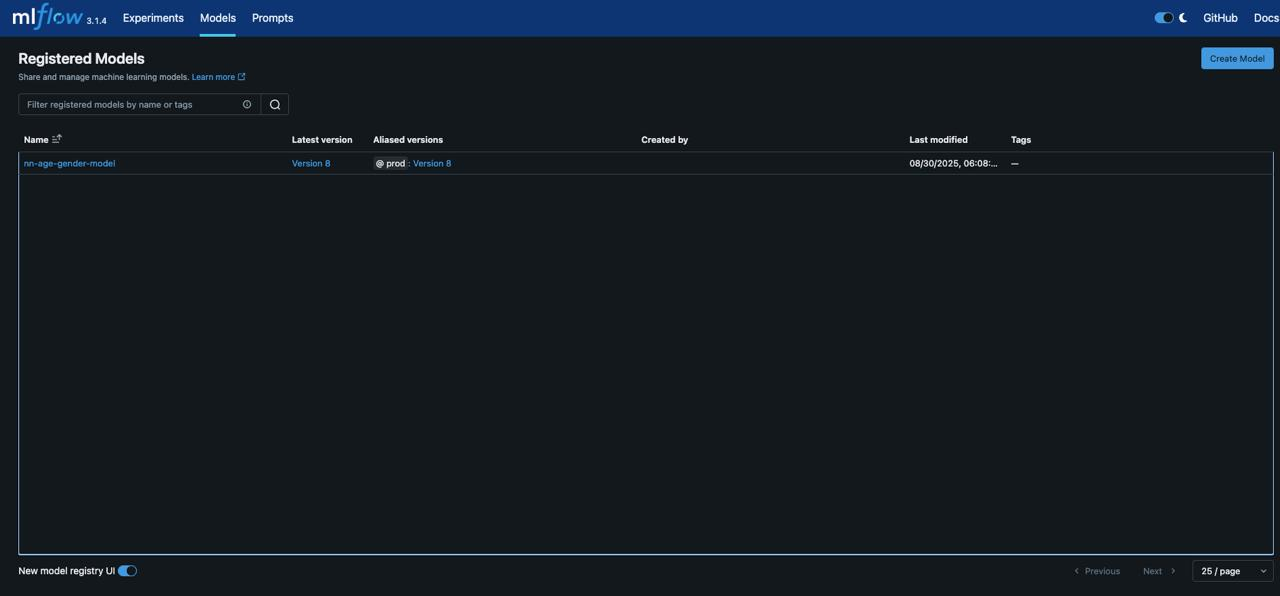
\includegraphics[width=0.5\textwidth]{images/mlflow_register.jpeg}
\centering
\caption{Modelo almacenado en el MLflow Model Registry.}
\label{fig:mlflow-model}
\end{figure}

\subsection{Testing automatizado}
Se incluyó un script de pruebas (\texttt{test\_api.py}) para verificar el correcto funcionamiento de la API (endpoints, respuestas esperadas, formatos JSON, etc.), contribuyendo a garantizar la robustez ante cambios o despliegues posteriores.

\subsection{Contenerización con Docker y orquestación}
Se definió un archivo \texttt{docker-compose.yml} que pone en marcha simultáneamente:
\begin{itemize}
  \item El servicio de base de datos (\texttt{db}),
  \item El servidor MLflow (\texttt{mlflow}),
  \item El entorno de entrenamiento (\texttt{trainer}), y
  \item La API para inferencia (\texttt{face-api}).
\end{itemize}
Esto facilita la configuración, el despliegue en local o en servidor, y la escalabilidad modular del sistema.

\subsection{Carga dinámica de modelos en producción}
Un aspecto clave del despliegue es la \textbf{conexión directa con el MLflow Model Registry}. 
Cuando el contenedor de la API se inicializa, consulta el servidor MLflow definido en la variable de entorno \texttt{MLFLOW\_TRACKING\_URI}. 
Luego solicita la versión del modelo registrada bajo el alias de producción (por ejemplo, \texttt{prod}), descarga ese artefacto y lo carga en memoria para realizar inferencias. 
De esta manera, la API siempre sirve el modelo más reciente validado, sin necesidad de reconstruir la imagen Docker. 
En caso de fallar la conexión, el sistema dispone de mecanismos de respaldo: carga un modelo guardado localmente o, en último recurso, un modelo dummy de prueba.

\subsection{Interfaz de producción: la API REST}
La API permite recibir imágenes, procesarlas (detección, preprocesamiento), ejecutar predicción y devolver los resultados de edad y género. 
Además, puede integrarse fácilmente en aplicaciones externas gracias a su diseño RESTful y a la arquitectura desacoplada.

\begin{figure}[h]
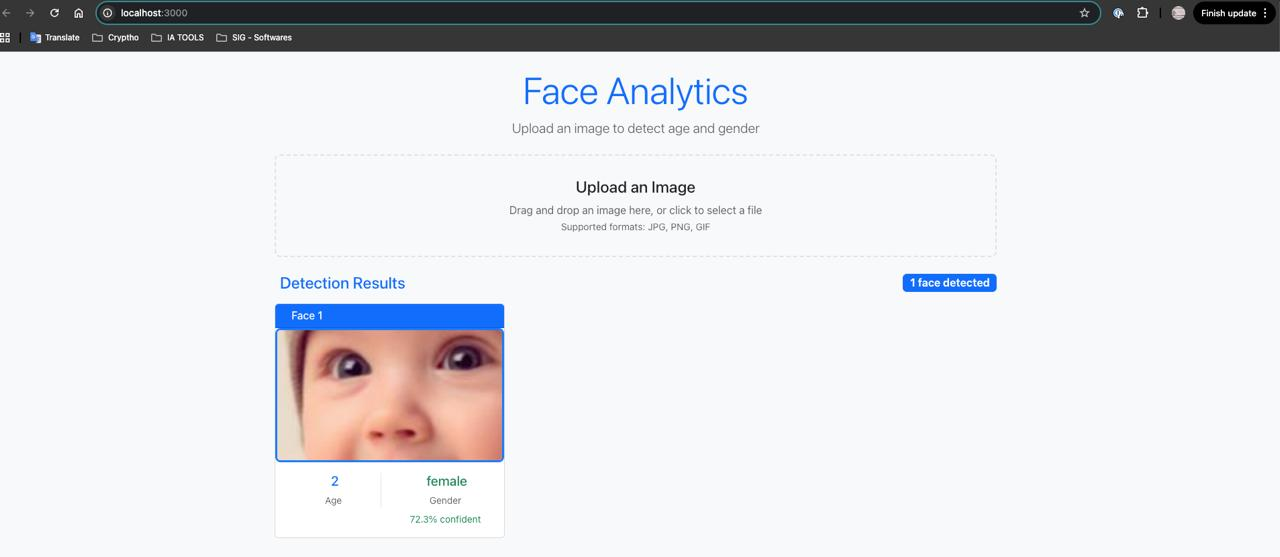
\includegraphics[width=0.5\textwidth]{images/frontend_project.jpeg}
\centering
\caption{Prueba de la API REST con una imagen de entrada y salida de edad/género.}
\label{fig:api-frontend}
\end{figure}

\subsection{Figura ilustrativa del pipeline}
Una figura complementaria (Figura~\ref{fig:deployment-architecture}) representa el flujo completo: 
desde el entrenamiento y registro en MLflow, pasando por la orquestación con Docker, hasta la consulta al Model Registry y la respuesta de predicción servida por la API.

\begin{figure}[h]
\centering
\includegraphics[width=0.5\textwidth]{images/pipeline_workflow.png}
\caption{Pipeline de despliegue: integración entre entrenamiento, MLflow y la API en producción.}
\label{fig:pipeline_workflow}
\end{figure}

\section{Pipeline}

\begin{table}[H]
\centering
\caption{Pipeline de MLOps implementado en el proyecto}
\label{tab:pipeline}
\begin{tabularx}{\linewidth}{|X|X|X|}
\toprule
\textbf{Etapa} & \textbf{Descripción} & \textbf{Implementación / Evidencia} \\
\midrule
\small \textbf{Ingesta de Datos} & Descarga y organización del dataset UTKFace, con fallback a datos sintéticos para pruebas locales. & Script \texttt{download\_utkface.py} (descarga desde Kaggle, genera imágenes sintéticas). \\
\midrule
\small \textbf{Preparación de Datos} & Extracción de anotaciones de edad y género a partir de la convención de nombres de los archivos. & Script \texttt{prepare\_utkface.py} (genera archivo \texttt{labels.csv} con metadatos). \\
\midrule
\small \textbf{Entrenamiento} & Entrenamiento multitarea para edad (regresión) y género (clasificación) con MobileNetV2 preentrenada, dos fases: extracción de características y fine-tuning. & Script \texttt{training.py} (Keras + MLflow, logging de métricas, guardado de artefactos y exportación ONNX). \\
\midrule
\small \textbf{Seguimiento y Registro} & Registro de parámetros, métricas, curvas de entrenamiento, matriz de confusión y modelos en formato TensorFlow/ONNX. & \textbf{MLflow Tracking} y \textbf{MLflow Model Registry} en contenedor dedicado. \\
\midrule
\small \textbf{Testing} & Validación automatizada del correcto funcionamiento de los endpoints de inferencia. & Script \texttt{test\_api.py}. \\
\midrule
\small \textbf{Despliegue en Producción} & Arquitectura distribuida con Docker Compose: base de datos, MLflow, entorno de entrenamiento y API REST. & \texttt{docker-compose.yml} (contenedores \texttt{db}, \texttt{mlflow}, \texttt{trainer}, \texttt{face-api}). \\
\midrule
\small \textbf{Inferencia en la API} & API REST en FastAPI que recibe imágenes, conecta al Model Registry de MLflow, descarga el modelo con alias de producción y expone predicciones de edad y género. & Clase \texttt{FaceAnalyticsService} en \texttt{face-api} (carga dinámica de modelos, funciones de predicción y embeddings). \\
\bottomrule
\end{tabularx}
\end{table}

% \newpage
\section{Conclusión}

Habiendo revisado de manera general las caracteristicas de ambos productos y
poninendo a prueba sus capacidades, recomendamos el uso de \textbf{Amazon API Gateway}
por las siguientes razones:
\begin{itemize}
  \item \textbf{Integración}
  \item \textbf{Facilidad de Uso}
  \item \textbf{Costos}
\end{itemize}
A su vez tambien reconocemos que el producto Kong podría ser una muy buena opción en
casos muy particulares, pero a nivel general recomendamos \textbf{Amazon API Gateway}


%%
%% The acknowledgments section is defined using the "acks" environment
%% (and NOT an unnumbered section). This ensures the proper
%% identification of the section in the article metadata, and the
%% consistent spelling of the heading.
% \begin{acks}
% To Robert, for the bagels and explaining CMYK and color spaces.
% \end{acks}

%%
%% The next two lines define the bibliography style to be used, and
%% the bibliography file.
\bibliographystyle{ACM-Reference-Format}
\bibliography{bibliography}


%%
%% If your work has an appendix, this is the place to put it.
\appendix

\end{document}
\endinput
%%
%% End of file `sample-sigplan.tex'.